\chapter{TileLink: A Substrate Protocol for Coherence Policy Transactions }
\label{c.tilelink}

TileLink is a protocol designed to be a substrate for cache coherence transactions implementing a particular cache coherence policy within an on-chip memory hierarchy.
Its purpose is to orthogonalize the design of the on-chip network and the implementation of the cache controllers from the design of the coherence protocol itself.

Any cache coherence protocol that conforms to TileLink's transaction structure can be used interchangeably with the physical networks and cache controllers we provide.

TileLink is roughly analogous to the data link layer in the IP network protocol stack, but exposes some details of the physical link necessary for efficient controller implementation.
It also codifies some transaction types that are common to all protocols, particularly the transactions servicing memory accesses made by agents that do not themselves have caches with coherence policy metadata.

\section{Background}

Transactional approach to coherence.

Shape of coherence transactions.

Client/Manager Architecture.

\section{Architecture}
\label{s.arch}

TileLink assumes a Client/Manager architecture.
Hierarchical.

Consists of agents and channels.

Four hop protocol.

What it is/is not for. 

TileLink tries to impose as few constraints as possible on the implementation of both the agents' controllers and the underlying physical network.
This design emphasis somewhat increases protocol complexity, but makes TileLink compatible with a wide variety of physical design constraints and application domains.
With regards to agents, TileLink does not make assumptions about what state the agents are capable of storing about each cache block (though it does require agents without state to operate in particular, conservative ways).
With regards to the underlying physical network, TileLink does not assume that messages are delivered in order between two particular endpoints (though it does require an extra transaction step if they are not ordered point-to-point).
The ramifications of these design decisions are discussed in more detail in the following sections.

\subsection{Agents}

Agents participating in the TileLink protocol are either:
\begin{description}
\item[Clients] that request access to cache blocks, or
\item[Managers] that oversee the propagation of cache block permissions and data.
\end{description}

A client may be a cache, a DMA engine, an accelerator, or any other component that would like to participate in performing memory operations that target the coherent abstraction of global shared memory.
Even clients that do not actually cache a copy of the data within themselves may use TileLink in order to see a coherent view of memory with respect to other clients that do have caches
(i.e. to see dirtied data currently stored in those clients).
Clients are responsible for initiating transactions to gain or cede permissions on copies of cache blocks, and also for reporting on whether they possess certain permissions on those blocks.

A manager may be an outer-level cache controller, a directory, or a broadcast medium such as a bus.
Managers may or may not posses a local copy of a data block themselves, but they must know how to supply data in response to clients' requests.
In addition to supplying data, managers are responsible for tracking which clients have been granted which permissions on a data block,
and for probing those clients in order to ensure that the 
single-writer, multiple-reader (SWMR) invariant \cite{sorin2011primer} is upheld.
If a manager does not track the specific condition of individual blocks, it must be pessimistic
in terms of the quantity and type of probe messages that it sends.
A manager also provides a point of serialization for coherence transactions
initiated by any of the clients within its domain.

In a multi-level memory hierarchy, a particular agent can function as both
a client (with respect to caches further out in the hierarchy)
and a manager (with respect to caches closer in to the processors).
Such an agent is termed {\em hierarchical}.
These agents must perform a translation of the various message types between the inner and outer protocol.
This translation process is described in more detail in Chapter~\ref{c.coh}.
Hierarchical agents may or may not store a copy of the data locally, but they must at least track a set of ongoing transactions and serve as a serialization point for the inner protocol.

\subsection{Channels}

TileLink defines five independent transaction channels.
These channels may be multiplexed over the same physical link, but to avoid deadlock TileLink specifies a priority amongst the channels that must be strictly enforced.
Channels may contain both metadata and data components.

The channels are:
\begin{description}
\item[Acquire.] Initiates a transaction to acquire access to a cache block with proper permissions. Also used to write data without caching it.
\item[Probe.] Queries a client to determine whether it has a cache block or revoke its permissions on that cache block.
\item[Release.] Acknowledgement of probe receipt, releasing permissions on the line along with any dirty data. Also used to voluntarily write back data.
\item[Grant.] Provides data or permissions to the original requestor granting, access to the cache block. Also used to acknowledge voluntary Releases.
\item[Finish.] Final acknowledgement of transaction completion from requestor, used for transaction ordering.
\end{description}

At present time, all channels are routed from clients to managers or from managers to clients. (In the future, client-to-client Grants may be added.)

The prioritization of channels is Finish >> Grant >> Release >> Probe >> Acquire.
Preventing messages of a lower priority from blocking messages of a higher priority from being sent or received is necessary to avoid deadlock.

\subsection{Transaction Flows}

There are two types of transaction that can occur on a cache block managed by TileLink.
The first type enables clients to acquire permissions on a cache block:
\begin{itemize}
\item A client sends an Acquire to a manager.
\item The manager sends any necessary Probes to clients.
\item The manager waits to receive a Release for every Probe that was sent.
\item The manager communicates with backing memory if required.
\item Having obtained the required data or permissions, the manager responds to the original requestor with a Grant.
\item Upon receiving a Grant, the original client responds to the manager with a Finish to complete the transaction.
\end{itemize}
After this transaction has completed, the client has acquired permissions to either read or write the cache block, as well as copy of the block's data.
If the manager is capable of tracking which

The second type of transaction is supports clients voluntarily releasing a cache block:
\begin{itemize}
\item A client sends a Release to a manager, specifying that it is voluntary.
\item The manager communicates with backing memory if required.
\item The manager acknowledges completion of the transaction using a Grant.
\end{itemize}



\subsection{Concurrency}

TileLink does not make any assumptions about the ordering of messages sent point-to-point over particular channels.
Therefore, concurrency must be managed by agents at several points in the system.
\begin{itemize}
\item A manager should not accept a request for a transaction on a block that is already in-flight for a different client (unless it knows how to merge the two transactions as discussed below). Specifically, the manager must wait until it has received a Finish from the original client in order to ensure proper ordering of any future Grants.
\item If client has an outstanding voluntary writeback transaction, it cannot respond to an incoming Probe request on that block with Releases until it receives a Grant from the manager acknowledging completion of the writeback.
\end{itemize}

Transactions can be merged in certain situations. 

One specific situation that must be handled by all manager agents is receiving a voluntary Release for a block which another client is currently attempting to Acquire.
The manager must accept the voluntary Release as well as any Releases resulting from Probe messages, and provide Grant messages to both clients before the transaction can be considered complete.

When running on networks that provide guaranteed ordering of messages between any client/manager pair, the Finish acknowledgment of a Grant (and the Grant acknowledgement of a voluntary Release) can be omitted.

\subsection{Metadata, Data, and Control Signals}

Every channel is wrapped in the Chisel.DecoupledIO interface, meaning that each contains ready and valid signals as well as the following signals.

Channels with data may send the data over multiple beats; the width of the underlying network is exposed to improve the efficiency of refilling data into caches whose data array rows are of a matching size.
The client controller that generates this message is responsible for generating multiple sequential messages and incrementing the addr\_beat field as it does so.

\section{Built-in Transactions}

There are seven built-in types of Acquire that are available to all clients that want to participate in the coherence protocol, even if they themselves will not keep cached copies of the data.
Because these transactions do not create a new private copy of the targeted cache block, they are termed ``uncached'' transactions. 
However, they still participate in the standard TileLink transaction flow, meaning that they will result in probes of other caches and return coherence answers.

The available uncached transactions are as follows:
\begin{description}
\item[Get.] Fetches a single beat of data from a cache block and returns only that beat
\item[GetBlock.] Fetches an entire cache block and serves it back to the requestor.
\item[GetPrefetch.]  Prefetches a cache block into the next-outermost level of the memory hierarchy with read permissions
\item[Put.] Writes up to a beat's worth of data to backing memory. Uses a write mask to determine which bytes contain valid write data
\item[PutBlock.] Writes out an entire cache block to backing memory
\item[PutPrefetch.]  Prefetches a cache block into the next-outermost level of the memory hierarchy with write permissions
\item[PutAtomic.] Performs an atomic memory op in the next-outermost level of the memory hierarchy. The maximum available operand size is 64b (sizes and opcodes per RISC-V atomic instructions).
\end{description}

The PutBlock message is unique among the built-in Acquires in that may contains multiple beats of data (if the cache block size is larger than TLDataBits).
The client controller that generates this message is responsible for generating multiple sequential PutBlock messages and incrementing the addr\_beat field as it does so.

There are five built-in types of Grant that are available to all managers that want to participate in the coherence protocol.
Because ``uncached'' transactions do not create a new private copy of the targeted cache block, we use these Grant types mostly as acknowledgements.
The available types are as follows:
\begin{description}
\item[GetDataBlock.] Full cache block in response to Acquire.GetBlock,
\item[GetDataBeat.] Single beat of data in response to Acquire.Get or Acquire.PutAtomic,
\item[PutAck.] Acknowledgement of Acquire.\{Put, PutBlock\}.
\item[PrefetchAck.] Acknowledgment of Acquire.\{GetPrefetch, PutPrefetch\}.
\item[VoluntaryAck.] Acknowledgement of any voluntary Release.
\end{description}

The GetDataBlock message may contains multiple beats of data (if the cache block size is larger than TLDataBits).
The manager controller that generates this message is responsible for generating multiple sequential GetDataBlockmessages and incrementing the addr\_beat field as it does so.

\begin{table}[ht]
\begin{center}
\begin{tabular}{|l|l|l|}
    \hline
    Acquire & Grant & Effect \\ \hline \hline
    Get & GetDataBeat & Copy data in to client \\ \hline
    GetBlock & GetDataBlock & Copy data in to client \\ \hline
    GetPrefetch & PrefetchAck & Fetch data to outer memory with read permissions \\ \hline
    Put & PutAck & Update data in outer memory \\ \hline
    PutBlock & PutAck & Update data in outer memory \\ \hline
    PutPrefetch & PrefetchAck & Fetch data to outer memory with write permissions \\ \hline
    PutAtomic & GetDataBeat & Update data in outer memory and return old value. \\ \hline
\end{tabular}
\end{center}
\caption{Overview of built-in, uncached transactions.}
\label{tab:uncached}
\end{table}

Table~\ref{tab:uncached} provides and overview of the built-in transactions and their effect on memory.
 
\subsection{Memory Model}

Weak memory consistency.

Client is in charge of not issuing multiple writes to individual addresses over un-ordered physical links.

\section{Channel Signal Descriptions}

This section details the specific signals contained in each channel of the TileLink protocol.

Every channel is wrapped in the Chisel.DecoupledIO interface, meaning that each contains ready and valid signals as well as the following signals.

Channels with data may send the data over multiple beats; the width of the underlying network is exposed to improve the efficiency of refilling data into caches whose data array rows are of a matching size.

\subsection{Acquire}

Initiates a transaction to acquire access to a cache block with proper permissions.
Also used to write data without caching it (acquiring permissions for the write as it does so).

PutDataBlock messages may contains multiple beats of data (if the cache block size is larger than TLDataBits).
The client controller that generates this message is responsible for generating multiple sequential Release messages and incrementing the addr\_beat field as it does so.

\begin{table}[ht]
\begin{center}
\begin{tabular}{|l|l|l|}
    \hline
    Name & Type & Purpose \\ \hline \hline
addr\_block & UInt & Physical address of the cache block, with block offset removed \\ \hline
client\_xact\_id & UInt & Client's id for the transaction \\ \hline
data & UInt & Client-sent data, used for Put transactions \\ \hline
addr\_beat & UInt & Offset of this beat's worth of data within the cache block \\ \hline
built\_in\_type & Bool & Whether the transaction is a built-in or custom type \\ \hline
a\_type & UInt & Type of the transaction. For built-in transactions, one of: \\
        &      & \{Get, GetBlock, GetPrefetch, Put, PutBlock, PutPrefetch, PutAtomic\}. \\
        &      &  Otherwise defined by the coherence protocol. \\ \hline
union & Union & Used to derive the following subfields: \\ \hline \hline
allocate & Bool & R/W: Hints whether to allocate data in outer caches \\
         &      & when servicing this request \\ \hline
op\_code & UInt & Memory op code (Read, Write, or AMO ALU op) \\ \hline
op\_size & UInt & A: Size of the AMO operands (Byte, Half, Word, Double) \\ \hline
addr\_byte & UInt & A: Address of the AMO operands within the block \\ \hline
amo\_shift\_bits & UInt & A: Number of bits to shift block to extract AMO operands \\ \hline
wmask & UInt & W: Byte write mask for Write op's data \\ \hline
\end{tabular}
\end{center}
\caption{Fields of the Acquire channel.}
\label{tab:acquire}
\end{table}

\subsection{Probe}

Queries an agent to determine whether it has a cache block or revoke its permissions on that cache block.

\begin{table}[ht]
\begin{center}
\begin{tabular}{|l|l|l|}
    \hline
    Name & Type & Purpose \\ \hline \hline
addr\_block & UInt & Physical address of the cache block, with block offset removed \\ \hline
p\_type & UInt & Transaction type, defined by coherence protocol \\ \hline
\end{tabular}
\end{center}
\caption{Fields of the Probe channel.}
\label{tab:probe}
\end{table}


\subsection{Release}

Acknowledgement of probe receipt, releasing permissions on the line along with any dirty data.
Also used to voluntarily write back data or cede permissions on the block.

Release messages may contains multiple beats of data (if the cache block size is larger than TLDataBits).
The client controller that generates this message is responsible for generating multiple sequential Release messages and incrementing the addr\_beat field as it does so.

\begin{table}[ht]
\begin{center}
\begin{tabular}{|l|l|l|}
    \hline
    Name & Type & Purpose \\ \hline \hline
addr\_block & UInt & Physical address of the cache block, with block offset removed \\ \hline
client\_xact\_id & UInt & Client's id for the transaction \\ \hline
data & UInt & Used to writeback dirty data \\ \hline
addr\_beat & UInt & Offset of this beat's worth of data within the cache block \\ \hline
r\_type & UInt & Transaction type, defined by coherence protocol \\ \hline
voluntary & Bool & Whether this release is voluntary or in response to a Probe \\ \hline
\end{tabular}
\end{center}
\caption{Fields of the Release channel.}
\label{tab:release}
\end{table}

\subsection{Grant}

Provides data or permissions to the original requester granting, access to the cache block. Also used to acknowledge voluntary Releases.

The GetDataBlock message may contains multiple beats of data (if the cache block size is larger than TLDataBits).
The manager controller that generates this message is responsible for generating multiple sequential GetDataBlockmessages and incrementing the addr\_beat field as it does so.

\begin{table}[ht]
\begin{center}
\begin{tabular}{|l|l|l|}
    \hline
    Name & Type & Purpose \\ \hline \hline
built\_in\_type & Bool & Whether transaction type is built-in or custom \\ \hline
g\_type & UInt & Type of the transaction. For built-in transactions, one of: \\
        &      & \{VoluntaryAck, PrefetchAck, PutAck, GetDataBeat, GetDataBlock\}. \\
        &      & Otherwise defined by the coherence protocol \\ \hline
client\_xact\_id & UInt & Client's id for the transaction \\ \hline
manager\_xact\_id & UInt & Manager's id for the transaction, passed to Finish \\ \hline
data & UInt & Used to supply data to original requestor \\ \hline
addr\_beat & UInt & Offset of this beat's worth of data within the cache block \\ \hline
\end{tabular}
\end{center}
\caption{Fields of the Grant channel.}
\label{tab:grant}
\end{table}


\subsection{Finish}

Final acknowledgement of transaction completion from requestor, used for transaction ordering.

\begin{table}[ht]
\begin{center}
\begin{tabular}{|l|l|l|}
    \hline
    Name & Type & Purpose \\ \hline \hline
manager\_xact\_id & UInt & Manager's id for the transaction \\ \hline
\end{tabular}
\end{center}
\caption{Fields of the Finish channel.}
\label{tab:finish}
\end{table}

\section{Agent-Specific Views of TileLink}

\begin{figure}[t!]
\centering
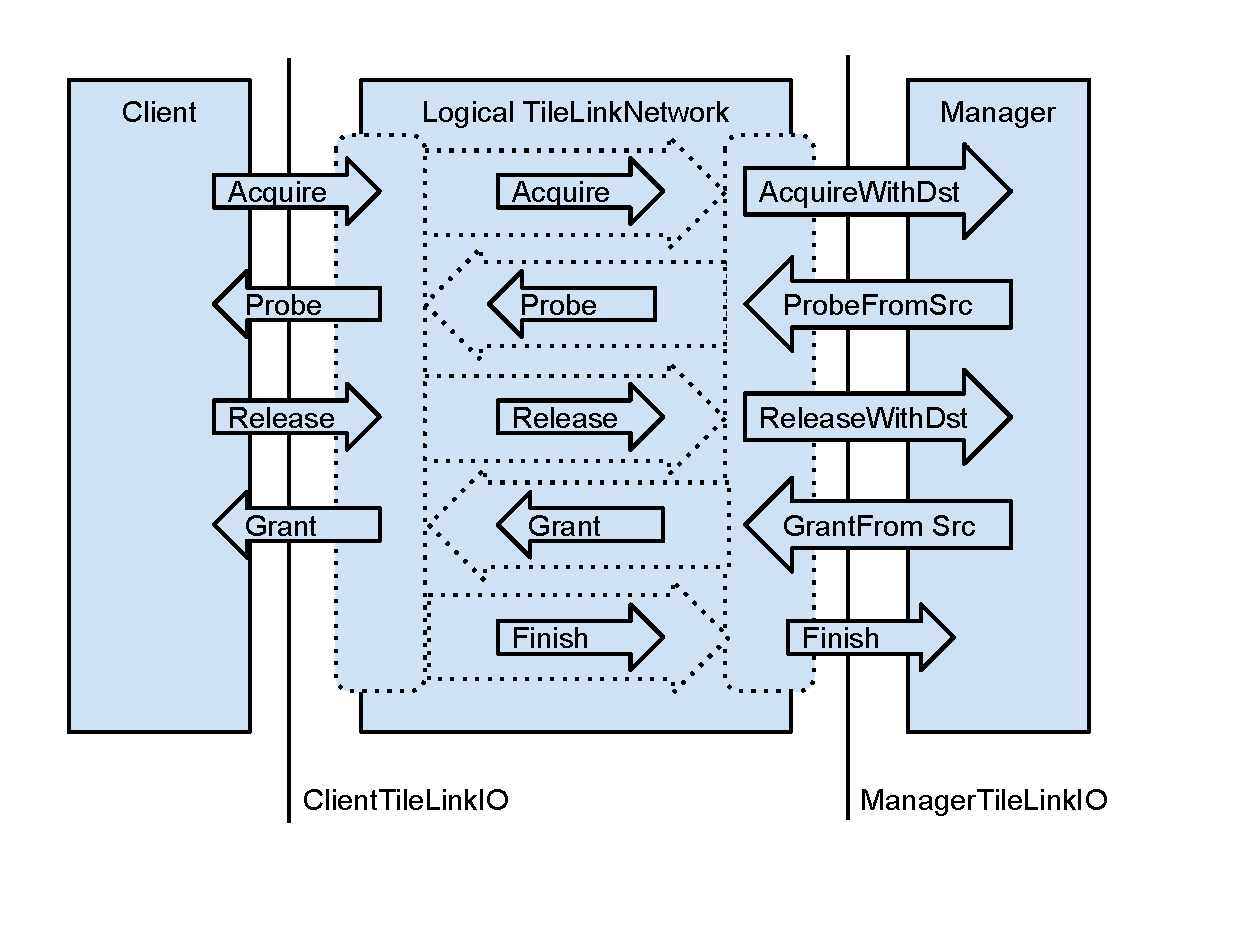
\includegraphics[width=1\columnwidth]{tilelink/figures/agent-specific.pdf}
\caption{Overview of the logic view of the TileLink interface presented to each type of agent.}
\label{fig:agent}
\end{figure}

For the convenience of designers implementing Client and Manager agents, we provide TileLinkNetworkPort modules which abstract away the details of the on-chip network implementation.
These network ports automatically generate networking headers, perform SerDes for narrower physical network channels, and generate appropriate control flow logic.
The ports then expose simplified subsets of the TileLink channels to the agent modules.
Figure~\ref{fig:agent} provides an overview of these two interfaces.

ClientTileLinkIO consists of standard Acquire, Probe, Release, and Grant message channels.
It does not include the Finish channel as generating those acknowledgements is handled by the ClientTileLinkNetworkPort.

ManagerTileLinkIO consists of Acquire, Probe, Release, and Grant message channels that have additional data appended about the source or destination of messages, expressed in terms of the Client's id.
It does include a Finish channel so that the manager knows when to register the transaction as complete.

\section{TileLink Parameters}

This section defines the parameters that are exposed by the TileLink to the top-level design.
All agents that implement TileLink should either work for all values of these parameters within the specified ranges, or should add Chisel.Constraints to the design to define functional limits on hem.

\begin{table}[ht]
\begin{center}
\begin{tabular}{|l|l|l|}
    \hline
Name & Type & Function \\ \hline \hline
TLId & String & Ids a TileLink in a multi-level hierarchy \\ \hline
TLCoherencePolicy & CoherencePolicy & Coherency policy used on this TileLink \\ \hline
TLNManagers & Int & Number of manager agents \\ \hline
TLNClients & Int & Number of client agents \\ \hline
TLNCachingClients & Int & Number of client agents that cache data \\ \hline
TLNCachelessClients & Int & Number of client agents that do not cache data \\ \hline
TLMaxClientXacts & Int & Max number of concurrent transactions per client \\ \hline
TLMaxClientsPerPort & Int & Max number of clients sharing a single network port \\ \hline
TLMaxManagerXacts & Int & Max number of concurrent transactions per manager \\ \hline
TLBlockAddrBits & Int & Address size \\ \hline
TLDataBits & Int & Amount of block data sent per beat, must be > 64b \\ \hline
TLDataBeats & Int & Number of beats per cache block \\ \hline
TLNetworkIsOrderedP2P & Boolean & Whether the underlying physical network \\
                      &         & preserved point-to-point ordering of messages \\ \hline
\end{tabular}
\end{center}
\caption{Fields of the Finish channel.}
\label{tab:finish}
\end{table}

\section{Discussion}

Bandwidth

Extensibility

Conversion to AXI and RapidIO

Future work
